\clearpage
\section{Results}
\label{sec:results}

The numerical example in this section is based on the initial capacities of the four major electricity producers in Germany from figure \ref{fig:capacities}. We estimate the potential investment behaviour for a three-period horizon. Longer time horizons are possible, but lead to a larger amount of computational time and do not add much more economic insight. We consider rea time horizon of nine years, where investment decision have to be taken in $t=0,3,6$. Market equilibria for the production decisions have to be obtained in each node, also including the set of terminal nodes $\mathcal{S}$ in $t=9$.  The uncertainty is modeled with the calibrated scenario tree in figure \ref{fig:intercept}.

\subsection{Scenario generation}

We use the proposed procedure in from section \ref{sec:scenario-generation} with an estimate of $6\%$ for the growth of the market volume, which corresponds to the CAGR for 2002-2006 obtained from \cite{Datamonitor2007}. The calibrated scenario tree for the highest price segment from table \ref{tab:marketsegments} can be seen in figure \ref{fig:intercept}.

\begin{figure}[htb]
  \centering
\caption{Demand function intercept $\alpha_n^6$ with growth rate $g=0.06$}
  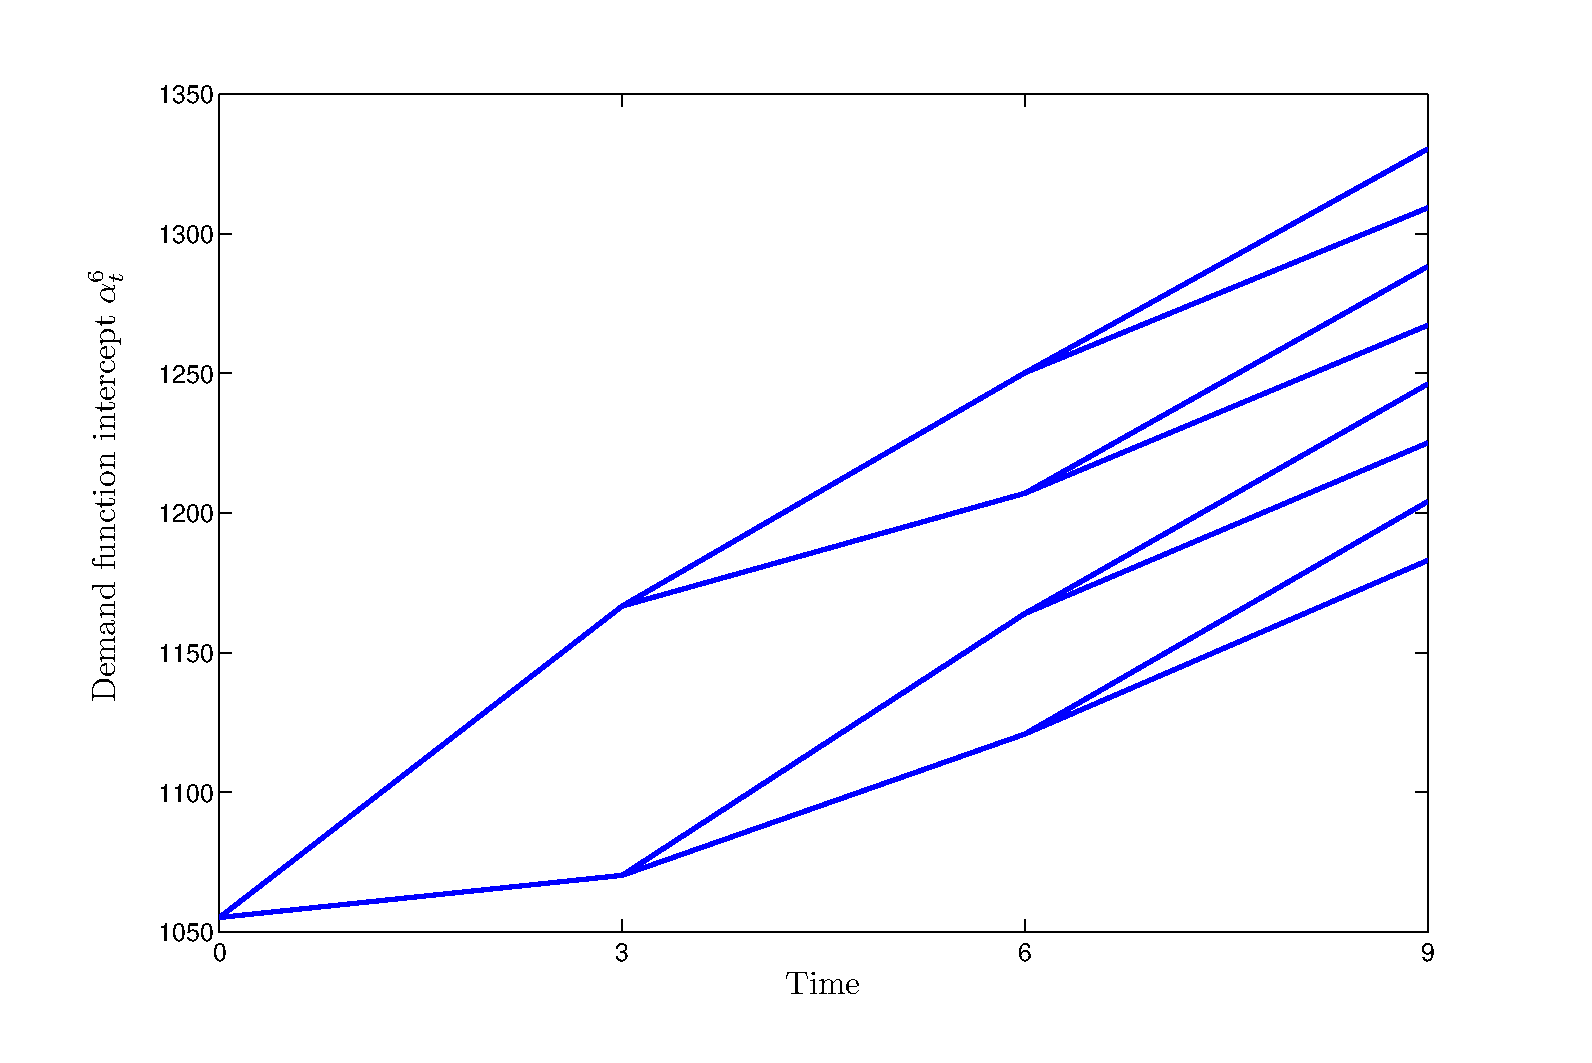
\includegraphics[width=0.75\textwidth]{numericalpaper/intercept}
  \label{fig:intercept}
\end{figure}

The intercepts for the other market states are calculated in an analogous manner. The slopes for the demand functions in each market state are given by \eqref{eq:demandslope}.

\subsection{Solution of the MCP}

We have implemented the mixed complementarity problem (MCP) in \eqref{eq:kkt_first}-\eqref{eq:kkt_last} in GAMS (General Algebraic Modelling System) and solved with with the PATH solver \citep[see][]{Ferris2000}.

Table \ref{tab:prod_init} shows the production quantities in the initial node. As mentioned before, the variables in the initial node are the so-called first-stage decision variables. We are primarily interested in these values, because the second-stage decision variables in the other nodes only reflect the recourse decision, i.e. the adoption to the uncertain development of the demand. The companies tend to produce more in market states with higher average prices and demand, see table \ref{tab:marketsegments}. 

\begin{table}[htb]
  \centering
  \caption{Production in the initial node $q_{i,0}^{m}$ (in MWh)}
  \label{tab:prod_init}
  \vspace{0.3cm}
  \begin{tabular}{rrrrrrr}
\hline
           &     $m=1$ &     $m=2$ &     $m=3$ &     $m=4$ &     $m=5$ &     $m=6$ \\
\hline\hline
       Rwe &    10,945.21  &    13,590.03  &    17,150.64  &    20,586.19  &    21,872.07  &    21,984.52  \\

       EON &    10,945.21  &    13,592.14  &    17,150.64  &    20,586.09  &    21,871.99  &    21,984.48  \\

    Vattenfall &    10,940.85  &    13,590.03  &    15,273.00  &    15,273.00  &    15,273.00  &    15,273.00  \\

      EnBW &    10,528.00  &    10,528.00  &    10,528.00  &    10,528.00  &    10,528.00  &    10,528.00  \\
\hline
  \end{tabular}
\end{table}

In table \ref{tab:invest_salv} we show the investment quantities in $t=0$ for various salvage value parameters. As expected, the investment quantities decrease when the parameter $\nu$ is lowered. Our results show that the two smaller players have an incentive to expand their generation capacity given the future expected demand growth. The larger players seem to have enough generation capacity at the moment, but of course investments are possible at later stages.

\begin{table}[htb]
  \centering
  \caption{Investment quantities in the initial node $I_{i,0}$ (in MW) with $\rho=0.025$}
  \label{tab:invest_salv}
  \vspace{0.3cm}
\begin{tabular}{rrrrr}
\hline
           &       $\nu=0.99$ &       $\nu=0.95$ &        $\nu=0.9$ &       $\nu=0.85$ \\
\hline\hline
 Vattenfall  &      5,015.93  &      4,832.23  &      4,626.18  &      4,516.54  \\

     EnBW  &      9,582.64  &      9,405.55  &      9,229.64  &      9,120.00  \\
\hline
\end{tabular}  
\end{table}


Next, we check the sensitivity of the investment quantities to a change in  the depreciation rate $\rho$. We see in table \ref{tab:invest_depr} that with higher depreciation the incentive to invest increases.

\begin{table}[htb]
  \centering
  \caption{Investment quantities in the initial node $I_{i,0}$ (in MW) with $\nu=0.95$}
  \label{tab:invest_depr}
  \vspace{0.3cm}
\begin{tabular}{rrrrr}
\hline
           &      $\rho=0.025$ &       $\rho=0.03$ &      $\rho=0.035$ &       $\rho=0.04$ \\
\hline\hline
Vattenfall &      4,832.23  &      4,908.60  &      4,984.96  &      5,061.33  \\

      EnBW &      9,405.55  &      9,458.19  &      9,510.83  &      9,563.47  \\
\hline
\end{tabular}  
\end{table}



%%% Local Variables: 
%%% mode: latex
%%% TeX-master: "gencapinvest"
%%% End: 
